\newpage
\noindent
\textbf{Beispiel 2} \\ \\
a) \\ \\
Skizze der auftretenden Kräfte
\begin{figure}[h]
	\centering
	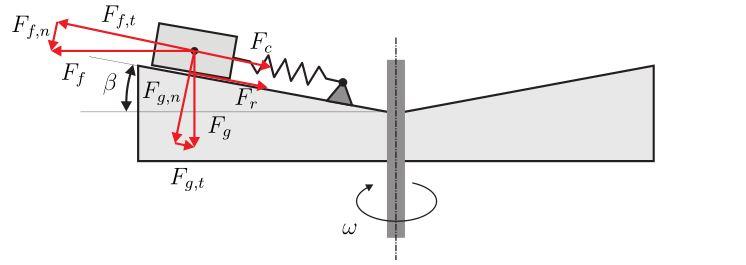
\includegraphics[width=12.5cm]{tikz/11_03_2016_2a}
\end{figure}
\newline
Hier treten die Fliehkraft
\[
	F_f = m(x_m + l)\cos\beta\omega^2
\]
die Gewichtskraft
\[	
	F_g = mg
\]
die Federkraft
\[
	F_c = c (x_m - x_0)
\]
und die Reibkraft (Haftreibung) 
\[
	F_r = (F_{g,n} + F_{f,n})\mu_H
\]
auf. Die einzelnen Terme der Reibkraft werden im nächsten Punkt genauer erklärt.\\ \\
b) \\ \\
Die einzelnen Komponenten der auftretenden Kräfte lauten
\begin{align*}
	F_{f,t} &= m(x_m + l)\cos\beta\omega^2 \\
	F_{f,n} &= m(x_m + l)\cos\beta\sin\beta\omega^2 \\
	F_{g,t} &= mg\sin\beta \\
	F_{g,n} &= mg\cos\beta
\end{align*}
c)\\ \\
Die beiden Haftbedingungen lauten
\begin{align*}
	F_{f,t} - F_{g,t} - F_c &> \mu_H (F_{g,n} + F_{f,n}) \rightarrow \text{Bewegung nach außen} \\
	F_{f,t} - F_{g,t} - F_c &< -\mu_H (F_{g,n} + F_{f,n}) \rightarrow \text{Bewegung nach innen}
\end{align*}
\newpage
\noindent
d) \\ \\ 
Die kritische Winkelgeschwindigkeit kann aus der ersten Haftbedingung wie folgt ermittelt werden.
\begin{align*}
	&F_{f,t} - F_{g,t} - F_c > \mu_H (F_{g,n} + F_{f,n}) \\
	&m(x_m + l)\cos\beta\omega^2 - mg\sin\beta - c(x_m - x_0) > \mu_H (mg\cos\beta + m(x_m + l\cos\beta\sin\beta\omega^2)) \\
	& \omega^2 > \frac{mg\sin\beta + c(x_m - x_0) + \mu_Hmg\cos\beta}{m(x_m + l)\cos\beta - \mu_Hm(x_m + l)\cos\beta\sin\beta} \\
	&\omega > \sqrt{\frac{mg\sin\beta + c(x_m - x_0) + \mu_Hmg\cos\beta}{m(x_m + l)\cos\beta - \mu_Hm(x_m + l)\cos\beta\sin\beta}} \\
	&\omega < - \sqrt{\frac{mg\sin\beta + c(x_m - x_0) + \mu_Hmg\cos\beta}{m(x_m + l)\cos\beta - \mu_Hm(x_m + l)\cos\beta\sin\beta}}
\end{align*} 